\documentclass[aspectratio=169]{beamer}
\usepackage{./tex_refs/style_pres}

\useoutertheme{infolines}

\title{Railway Track Fault Detection}
\subtitle{Mathemathical Modeling Practice}
\author{Tamás DEMUS (XP4B9D)}
\date{Fall Semester 2022}

\begin{document}
\maketitle

\begin{frame}{Table of Contents}
    \tableofcontents
\end{frame}

\section{Dataset introduction and Problem Statement}
\begin{frame}{Dataset introduction and Problem Statement}
    \begin{columns}[c]
        \column{.45\textwidth}
        \begin{exampleblock}{Example images}
            \begin{columns}[c]
                \column{.45\textwidth}
                \includegraphics[height=2.2cm]{./data/Train/Non defective/1.jpg}
                \includegraphics[height=2.2cm]{./data/Train/Non defective/22.jpg}
                \centering
                Non defective
                \column{.45\textwidth}
                \includegraphics[height=2.2cm]{./data/Train/Defective/152.jpg}
                \includegraphics[height=2.2cm]{./data/Train/Defective/220.jpg}
                \centering
                Defective
            \end{columns}
        \end{exampleblock}
        \column{.45\textwidth}
        \begin{block}{}
            \begin{table}[!ht]
                \begin{tabular}{l c}
                    Dataset type & Number of images \\
                    \hline
                    Training     & 2x150            \\
                    Validation   & 2x31             \\
                    Test         & 2x11             \\
                \end{tabular}
            \end{table}
            \begin{enumerate}[label=Q\arabic*]
                \item \label{itm:Q1} What kind of defects are represented in the images?
                \item \label{itm:Q2} Can these defects detected by applying image manipulation
                      and machine learning approach?
                \item \label{itm:Q3} What accuracy rate can be achieved with the algorithm?
            \end{enumerate}
        \end{block}
    \end{columns}
\end{frame}

\begin{frame}{Defect types}
    \begin{columns}[b]
        \column{.30\textwidth}
        \centering
        \includegraphics[width=0.8\textwidth]{./data/Train/Defective/170.jpg}
        Cracked rail
        \column{.30\textwidth}
        \centering
        \includegraphics[width=0.8\textwidth]{./data/Train/Defective/181.jpg}
        Disjoint rails
        \column{.30\textwidth}
        \centering
        \includegraphics[width=0.8\textwidth]{./data/Train/Defective/260.jpg}
        Surface pitting
    \end{columns}
    \begin{columns}[c]
        \column{.30\textwidth}
        \centering
        \includegraphics[width=0.8\textwidth]{./data/Train/Defective/230.jpg}
        Missing spring
        \column{.30\textwidth}
        \centering
        \includegraphics[width=0.8\textwidth]{./data/Train/Defective/190.jpg}
        Missing fastener
    \end{columns}
\end{frame}

\section{Convolutional Neural Networks}
\begin{frame}{Convolutional Neural Networks}
    \begin{columns}[T]
        \column{0.4\textwidth}
        \begin{block}{Timeline}
            \begin{tabular}{r |@{\hspace{-2.7pt}$\bullet$ \hspace{5pt}} l}
                1989 & ConvNet              \\
                1998 & {\color{red}LeNet}   \\
                2012 & {\color{red}AlexNet} \\
                     & GoogleNet            \\
                2014 & Inception            \\
                     & {\color{red}VGG}     \\
                2015 & {\color{red}ResNet}  \\
                2016 & DenseNet             \\
                2017 & ResNeXt              \\
                2018 & Channel Boosted CNN  \\
                2019 & EfficientNet         \\
            \end{tabular}
        \end{block}
        \column{0.55\textwidth}
        \begin{block}{Settings}
            \begin{tabular}{l l}
                Optimizer         & Adam                    \\
                Loss function     & Binary crossentropy     \\
                Learning rate     & Manually tuned          \\
                Callbacks         & ModelCheckPoint         \\
                                  & EarlyStopping           \\
                                  & ReduceLROnPlateau       \\
                Data augmentation & Separated from pipeline \\
                                  & 2x25 images             \\
                                  & Rotation, Zoom          \\
            \end{tabular}
        \end{block}
    \end{columns}
\end{frame}

\section{Results}
\begin{frame}{Results}
    \begin{columns}[T]
        \column{0.45\textwidth}
        \begin{block}{LeNet-5}
            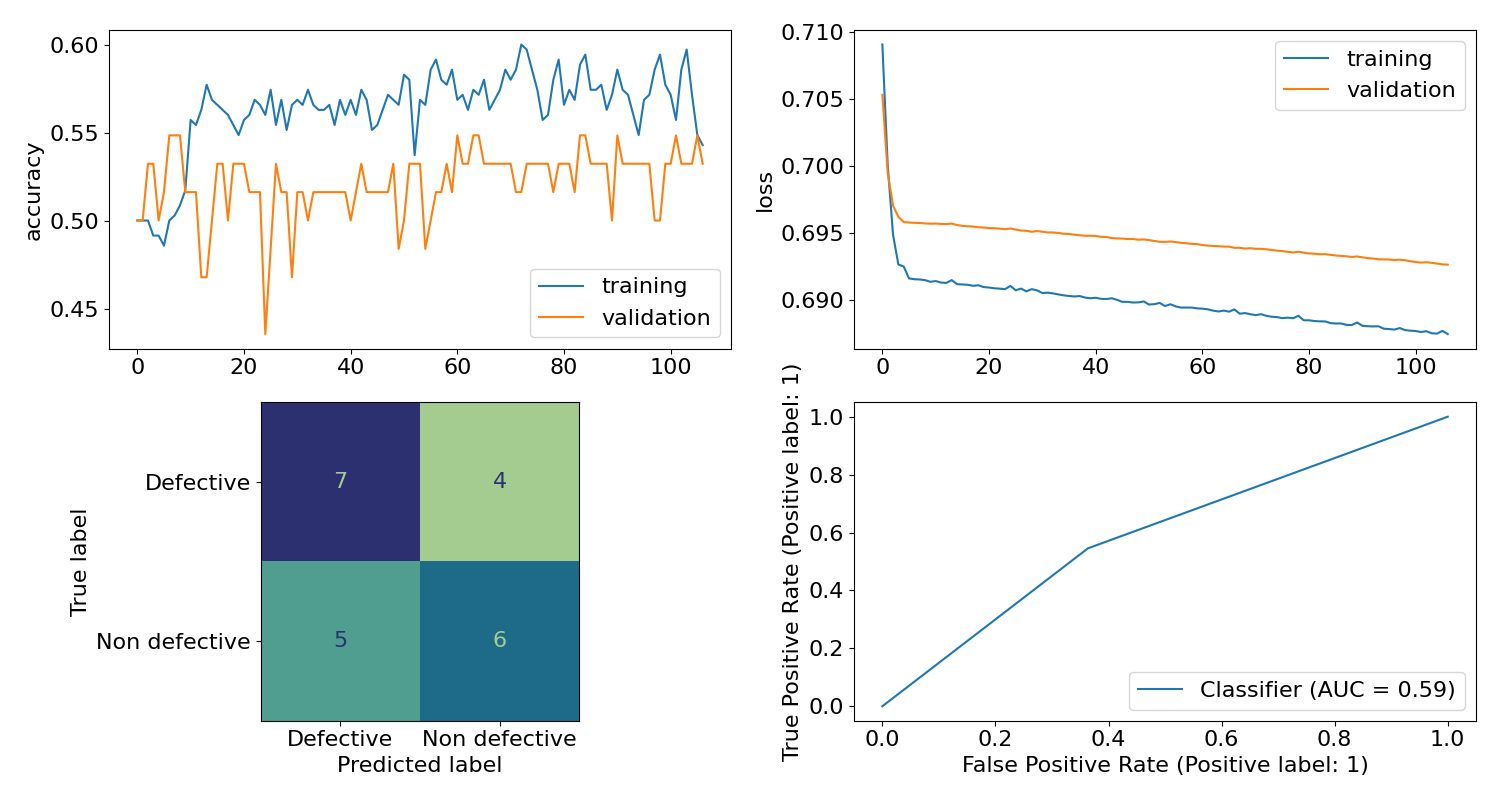
\includegraphics[width=\textwidth]{./tex_graphs/metrics_LeNet-5}
        \end{block}
        \column{0.45\textwidth}
        \begin{block}{AlexNet}
            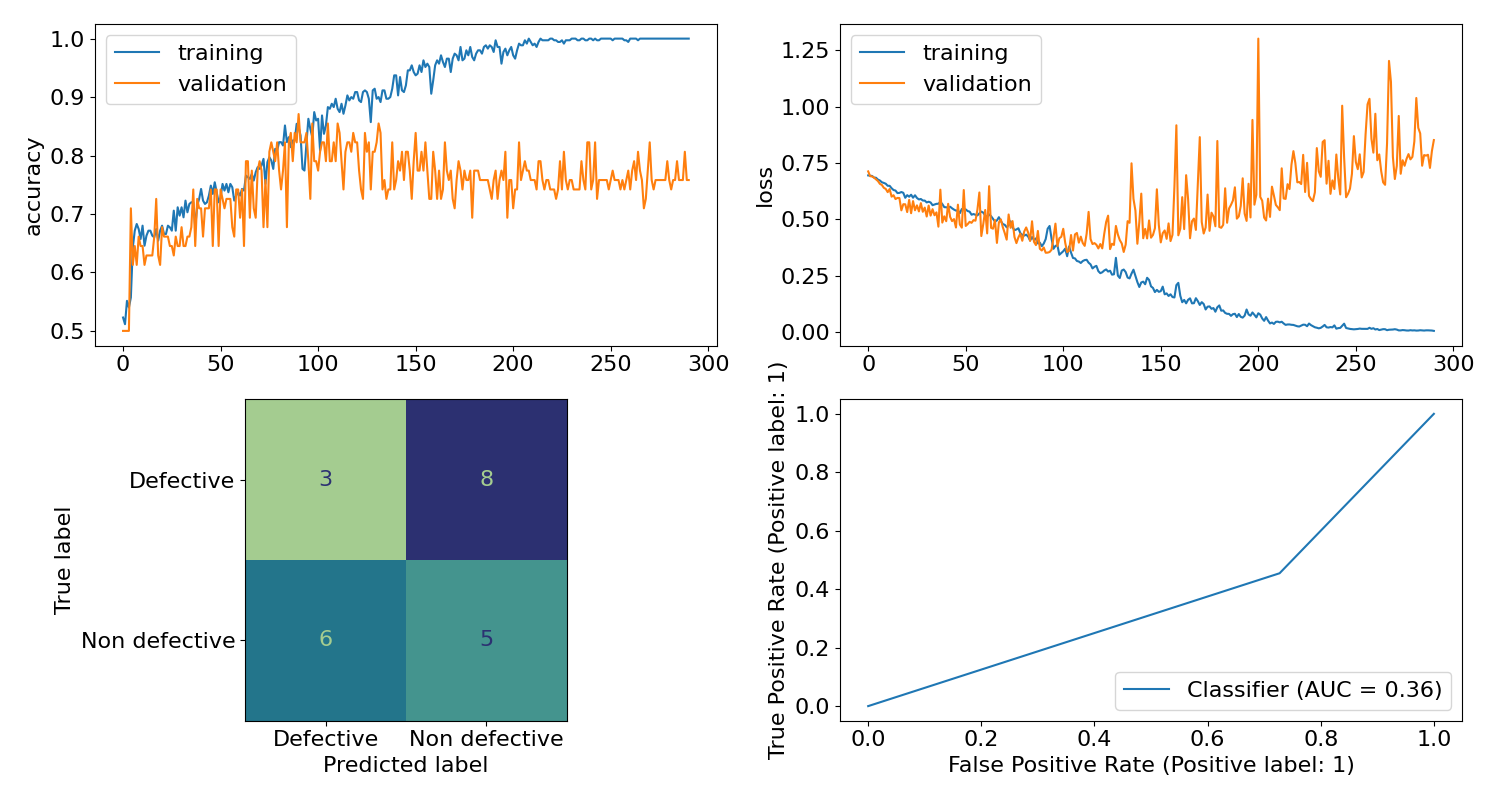
\includegraphics[width=\textwidth]{./tex_graphs/metrics_AlexNet}
        \end{block}
    \end{columns}
\end{frame}
\begin{frame}{Results}
    \begin{columns}[T]
        \column{0.45\textwidth}
        \begin{block}{VGG16}
            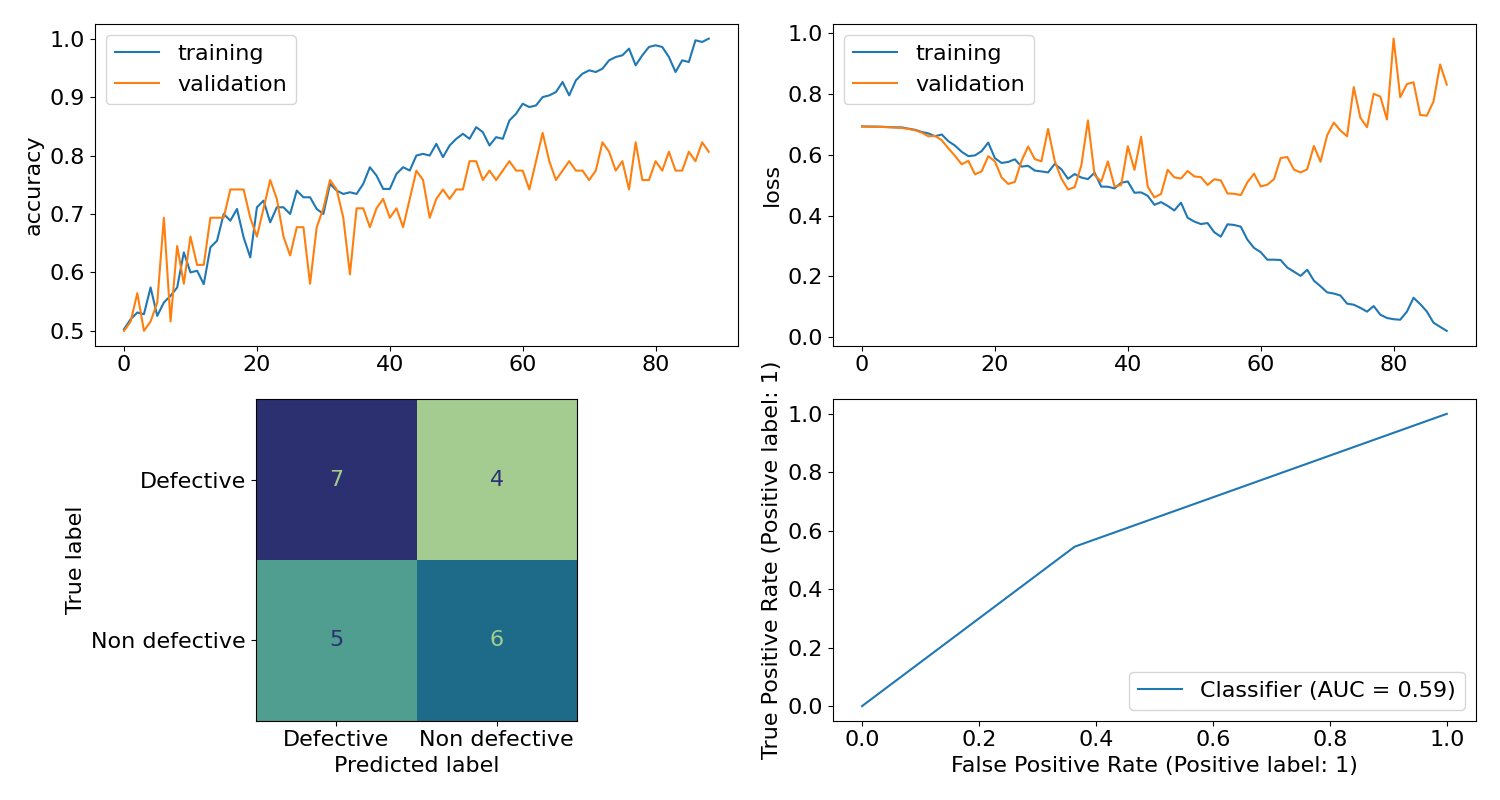
\includegraphics[width=\textwidth]{./tex_graphs/metrics_VGG16}
        \end{block}
        \column{0.45\textwidth}
        \begin{block}{Pretrained VGG16}
            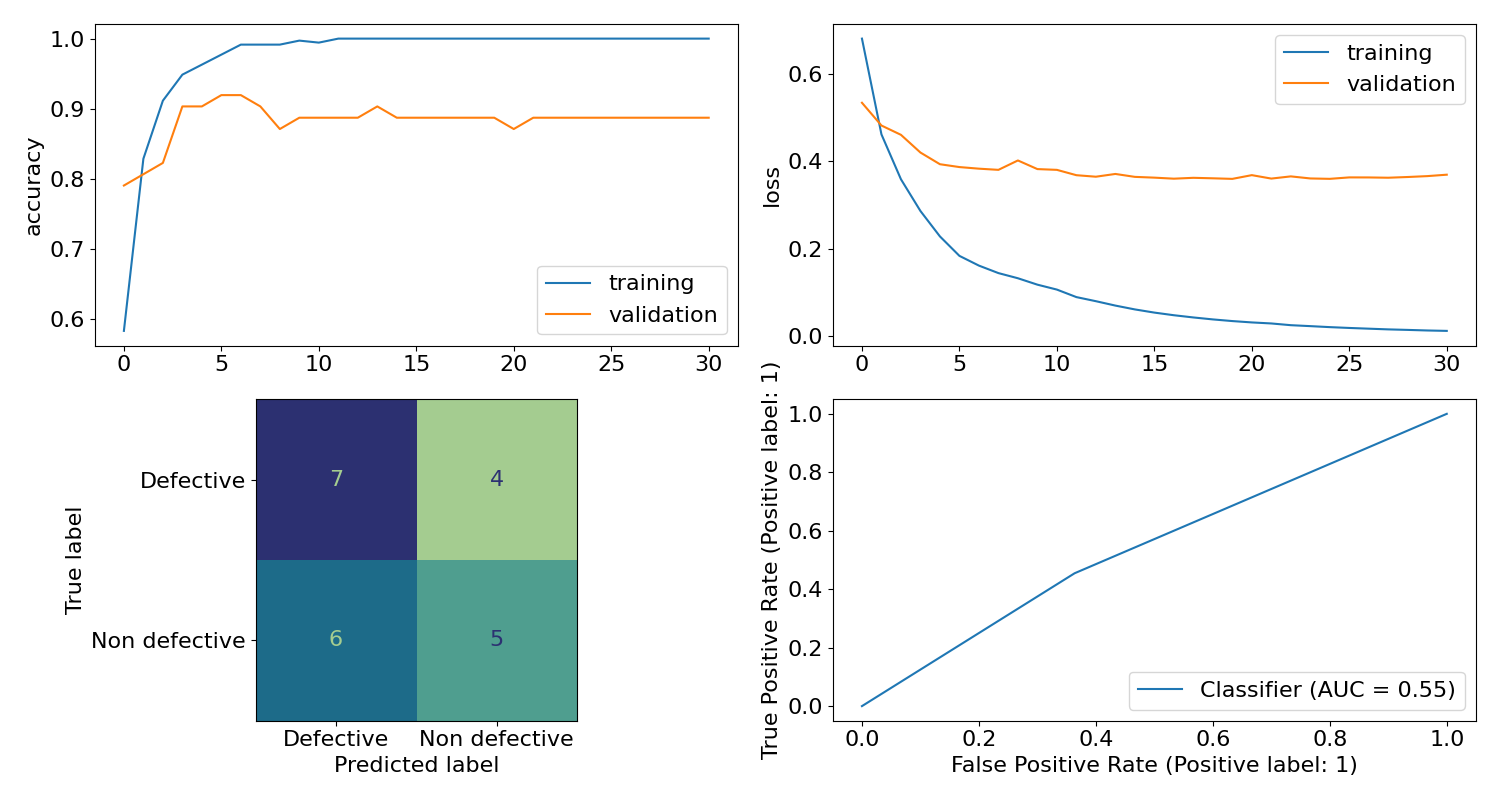
\includegraphics[width=\textwidth]{./tex_graphs/metrics_VGG16_pretrained.png}
        \end{block}
    \end{columns}
\end{frame}
\begin{frame}{Results}
    \begin{columns}[T]
        \column{0.45\textwidth}
        \begin{block}{Pretrained ResNet50}
            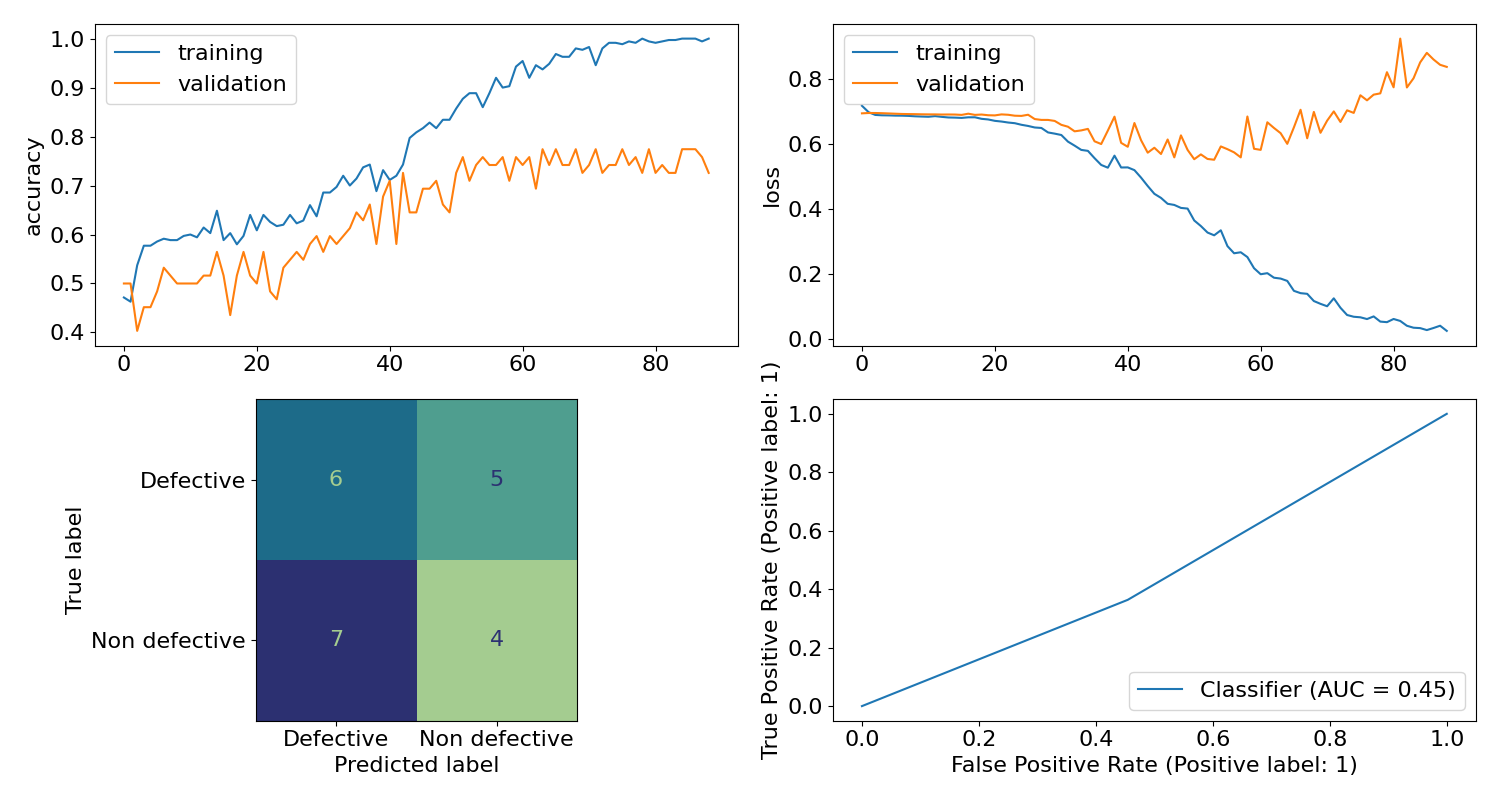
\includegraphics[width=\textwidth]{./tex_graphs/metrics_ResNet50_pretrained}
        \end{block}
        \column{0.45\textwidth}
        \begin{block}{Fine-tuned ResNet50}
            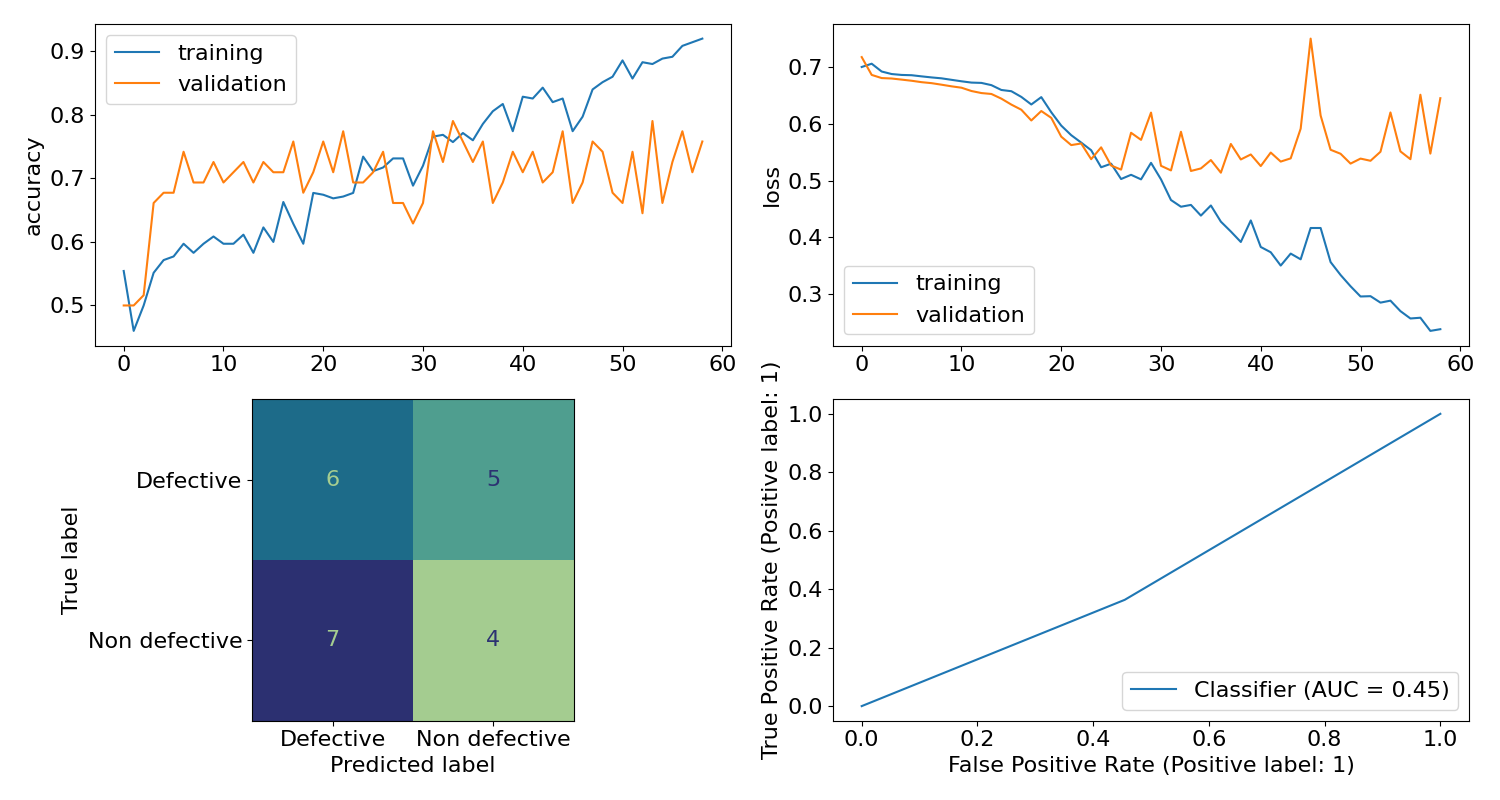
\includegraphics[width=\textwidth]{./tex_graphs/metrics_ResNet50_pretrained_finetuned.png}
        \end{block}
    \end{columns}
\end{frame}

\section{Hypertuning and bootstrapping}
\begin{frame}{}
    \begin{columns}
        \column{0.45\textwidth}
        \begin{block}{Hypertuning}
            \begin{itemize}
                \item Find best fit on validation dataset
                \item RandomSearch on Learning Rate
            \end{itemize}
        \end{block}
        \column{0.45\textwidth}
        \begin{block}{Bootstrapping}
            \begin{itemize}
                \item Mitigate representativeness issue
                \item 10 iterations with best LR
            \end{itemize}
        \end{block}
    \end{columns}
    \centering
    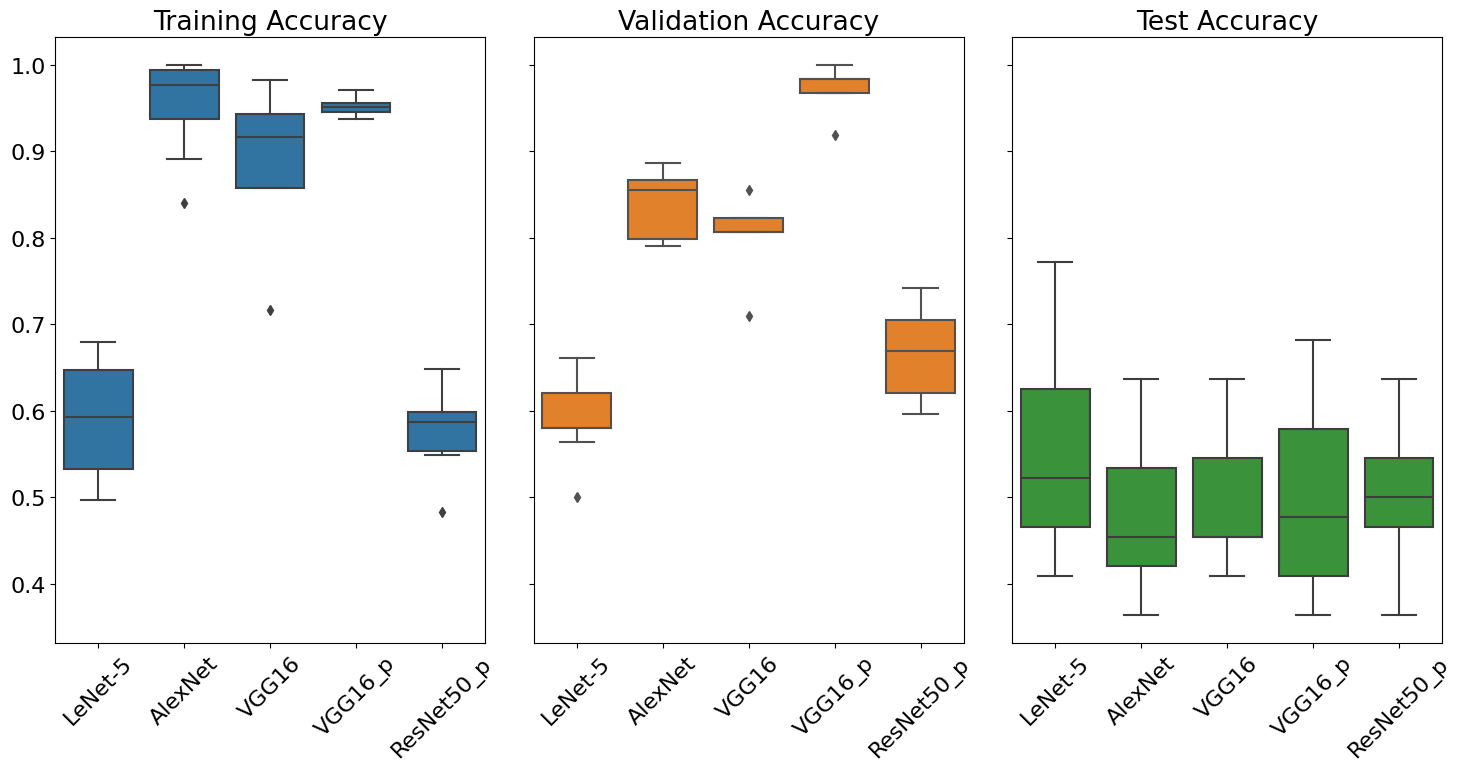
\includegraphics[height=5.5cm]{./tex_graphs/bootstrap_results.png}
\end{frame}

\section{Conclusion and further steps}
\begin{frame}{}
    \begin{columns}[T]
        \column{0.45\textwidth}
        \begin{block}{Conclusion}
            \begin{itemize}
                \item
            \end{itemize}
        \end{block}
        \column{0.45\textwidth}
        \begin{block}{Further steps}
            \begin{itemize}
                \item Hypertuning further parameters
                \item Data augmentation in pipeline
                \item Weight initialization
                \item Additional models: VGG19, ResNet34
                \item ResNet fine-tuning
            \end{itemize}
        \end{block}
    \end{columns}
\end{frame}

\begin{frame}
    \centering \Large
    Thank you very much for your kind attention!
\end{frame}
\end{document}